\documentclass[10pt]{article}
% \usepackage{geometry}
% \geometry{margin=0.2in}
\usepackage[utf8]{inputenc}

\nonstopmode
% \usepackage{minted}[cache=false]
\usepackage{graphicx} % Required for including pictures
\usepackage[figurename=Figure]{caption}
\usepackage{float}    % For tables and other floats
\usepackage{amsmath}  % For math
\usepackage{amssymb}  % For more math
\usepackage{fullpage} % Set margins and place page numbers at bottom center
\usepackage{paralist} % paragraph spacing
\usepackage{subfig}   % For subfigures
%\usepackage{physics}  % for simplified dv, and 
\usepackage{enumitem} % useful for itemization
\usepackage{siunitx}  % standardization of si units
\usepackage{hyperref}
% \usepackage{mmacells}
% \usepackage{listings}
% \usepackage{svg}
% \usepackage{xcolor, soul}
% \usepackage{bm}
\usepackage{braket}

% \usepackage{setspace}
% \usepackage{listings}
% \usepackage{listings}
% \usepackage[autoload=true]{jlcode}
% \usepackage{pygmentize}

% \definecolor{cambridgeblue}{rgb}{0.64, 0.76, 0.68}

% \sethlcolor{cambridgeblue}

\usepackage[margin=1.8cm]{geometry}
\newcommand{\C}{\mathbb C}
\newcommand{\D}{\bm D}
\newcommand{\R}{\mathbb R}
\newcommand{\Q}{\mathbb Q}
\newcommand{\Z}{\mathbb Z}
\newcommand{\N}{\mathbb N}
\newcommand{\PP}{\mathbb P}
\newcommand{\A}{\mathbb A}
\newcommand{\F}{\mathbb F}
\newcommand{\1}{\mathbf 1}
\newcommand{\ip}[1]{\left< #1 \right>}
\newcommand{\abs}[1]{\left| #1 \right|}
\newcommand{\norm}[1]{\left\| #1 \right\|}

\def\Tr{{\rm Tr}}
\def\tr{{\rm tr}}
\def\Var{{\rm Var}}
\def\calA{{\mathcal A}}
\def\calB{{\mathcal B}}
\def\calD{{\mathcal D}}
\def\calE{{\mathcal E}}
\def\calG{{\mathcal G}}
\def\from{{:}}
\def\lspan{{\rm span}}
\def\lrank{{\rm rank}}
\def\bd{{\rm bd}}
\def\acc{{\rm acc}}
\def\cl{{\rm cl}}
\def\sint{{\rm int}}
\def\ext{{\rm ext}}
\def\lnullity{{\rm nullity}}
\DeclareSIUnit\clight{\text{\ensuremath{c}}}
\DeclareSIUnit\fm{\femto\m}
\DeclareSIUnit\hplanck{\text{\ensuremath{h}}}


% \lstdefinelanguage{julia}%
%   {morekeywords={abstract,break,case,catch,const,continue,do,else,elseif,%
%       end,export,false,for,function,immutable,import,importall,if,in,%
%       macro,module,otherwise,quote,return,switch,true,try,type,typealias,%
%       using,while},%
%    sensitive=true,%
% %    alsoother={$},%
%    morecomment=[l]\#,%
%    morecomment=[n]{\#=}{=\#},%
%    morestring=[s]{"}{"},%
%    morestring=[m]{'}{'},%
% }[keywords,comments,strings]%

% \lstset{%
%     language         = Julia,
%     basicstyle       = \ttfamily,
%     keywordstyle     = \bfseries\color{blue},
%     stringstyle      = \color{magenta},
%     commentstyle     = \color{ForestGreen},
%     showstringspaces = false,
% }

% $
\begin{document}
\begin{center}
	\hrule
	\vspace{.4cm}
	{\textbf { \large CAS PY 452}}
\end{center}
Emmy Blumenthal \hspace{\fill} \hspace{\fill}  \textbf{} Discussion Notes\  \\
\textbf{Date:}\  Oct 19, 2022   \hspace{\fill} \textbf{Email:}\ emmyb320@bu.edu

\vspace{.4cm}
\hrule

\section*{Variational method for the hydrogen atom}

\paragraph{Problem statement:}

The hydrogen atom Hamiltonian is,
\begin{align}
	\hat H 
	=
	-
	\frac{\hbar^2}{2m_e}
	\nabla^2
	-
	\frac{e^2}{4 \pi \epsilon_0 r},
\end{align}
where we have used the approximation $m_\text{nucleus} \gg m_e$, where $m_e$ is the mass of the electron.
Use the following two ansatzes in order to estimate the ground state wavefunction and the ground state energy using the variational method:
\begin{align}
	\psi_e(r,\theta,\phi) &= A
	e^{-r/a}
	\\
	\psi_g(r,\theta,\phi)
	&=B
	e^{-(r/a)^2},
\end{align}
where $A,B$ are normalization constants.

\paragraph{Solution:}
First, we find the normalization constants by using integration by parts twice.
The relevant product rule calculations are,
\begin{align}
	-\frac{a}{2}\frac{d}{dr} (e^{-2r/a}r^2)
	=
	e^{-2r/a}r^2
	-
	ae^{-2r/a}r.
	\qquad
	-\frac{a}{2}\frac{d}{dr}(e^{-2r/a}r)
	=
	-\frac{a}{2}e^{-2r/a}
	+
	 r e^{-2r/a}
\end{align}
\begin{align}
	\iint
	\int_0^\infty 
	&\nonumber|\psi_e|^2 r^2  \, \mathrm{d}r\, \mathrm{d}\Omega
	=
	4\pi |A|^2\int_0^\infty e^{-2r/a} r^2  \, \mathrm{d}r
	=
	4\pi |A|^2
	\left(
	\left.-\frac{a}{2} e^{-2r/a}r^2\right|_{r=0}^{r \to \infty}
	+
	a \int_{0}^\infty e^{-2r/a} r
	\,
	\mathrm{d}r
	\right)
	\\
	&=
	4\pi |A|^2
	\left(
	0
	+
	a 
	\left[
		\left.-\frac{a}{2}
		e^{-2r/a}r
		\right|_{r=0}^{r\to \infty}
	+\frac{a}{2}
	\int_0^\infty
	e^{-2r/a}
	\,\mathrm{d}r
	\right]
	\right)
	=
	4\pi |A|^2 
	\frac{a^2}{2}
	\frac{a}{2}
	=
	\pi |A|^2 a^3\\
	\pi |A|^2 a^3 &= 1 \implies A=\frac{1}{\sqrt{a^3 \pi}}
	% \int_0^\infty e^{-2r/a} r^2  \, dr
\end{align}
\begin{align}
	-\frac{a^2}{4}
	\frac{d}{dr}(r e^{-2(r/a)^2})
	=
	r^2 e^{-2(r/a)^2}
	-
	\frac{a^2}{4}
	e^{-2(r/a)^2}
	% \qquad
	% -\frac{a^2}{4}
	% \frac{d}{dr}
	% (e^{-2(r/a)^2})
	% =
	% r e^{-2(r/a)^2}.
\end{align}
\begin{align}
	% \int_0^{2\pi}
	% \int_0^{\pi}
	\iint
	\int_0^{\infty}&\nonumber
	\left|\psi_g\right|^2r^2 \,\mathrm{d}r 	\,\mathrm{d}\Omega
	=
	4\pi |B|^2
	\int_0^\infty e^{-2(r/a)^2}r^2 \,\mathrm{d}r
	=
	4\pi |B|^2
	\times
	\frac{a^2}{4}
	\left(
	-\left.r e^{-2(r/a)^2}\right|_{r=0}^{r \to \infty}
	+
	\int_0^\infty e^{-2(r/a)^2} \,\mathrm{d}r
	\right)
	\\
	&=
	\pi a^2 |B|^2
	\left(
		-0
		+
		\frac{1}{2}
		\times
		\frac{a}{\sqrt{2}}
		\int_{-\infty}^\infty
		e^{-u^2}
		du
	\right)
	=
	a^3 |B|^2 (\pi/2)^{3/2}\\
	&
	a^3 |B|^2 (\pi/2)^{3/2} = 1
	\implies
	B = \left(
		\frac{2}{\pi a^2}
	\right)^{3/4}
\end{align}
The variational method lets us find an upper bound on the ground state energy and an approximate ground state wave-function by minimizing the energy functional $\braket{\psi | \hat H | \psi}$ over states $\ket{\psi}$.
To compute the energy functional, we act on our ansatz states $\psi_e, \psi_g$ with the Hamiltonian.
First recall that the spherical Laplacian when acting on a function with no angular dependence is,
\begin{align}
	\nabla^2 f(r)
	=
	\frac{\partial^2 f}{\partial r^2}
	+
	\frac{2}{r} \frac{\partial f}{\partial r},
\end{align}
so we find:
\begin{align}
	\hat H [\psi_e]/A
	&=
	-\frac{\hbar^2}{2m_e}
	\left(
	\frac{1}{a^2}e^{-r/a}
	-
	\frac{2}{ar}
	e^{-r/a}
	\right)
	-
	\frac{e^2}{4 \pi \epsilon_0 r}
	e^{-r/a}
	=
	-\frac{\hbar^2}{2ma^2}
	e^{-r/a}
	+
	\left(
		\frac{\hbar^2}{ma}
		-
		\frac{e^2}{4\pi \epsilon_0}
	\right)
	\frac{e^{-r/a}}{r}
	\\
	\hat H[\psi_g]/B
	&
	=
	-
	\frac{\hbar^2}{2m_e}\left(
		\frac{4r^2}{a^4}
		e^{-(r/a)^2}
		-
		\frac{6}{a^2}
		e^{-(r/a)^2}
	\right)
	-
	\frac{e^2}{4\pi\epsilon_0r}
	e^{-(r/a)^2}
	=
	\frac{3\hbar^2}{ma^2}
	e^{-(r/a)^2}
	-
	\frac{2\hbar^2}{m a^4}
	r^2e^{-(r/a)^2}
	-
	\frac{e^2}{4\pi \epsilon_0}
	\frac{e^{-(r/a)^2}}{r}
\end{align}
Next, we compute the inner products:
\begin{align}
	\braket{\psi_e | \hat H |\psi_e}
	&=\nonumber
	\iint 
	\int_0^\infty 
	\psi_e^* \hat H[\psi_e]
	r^2
	\,\mathrm{d}r
	\,\mathrm{d}\Omega 
	=
	4\pi A^2
	\left[
	-\frac{\hbar^2}{2ma^2}
	\int_0^\infty r^2   e^{-2r/a} \,\mathrm{d}r
	+
	\left(
		\frac{\hbar^2}{ma}
		-
		\frac{e^2}{4\pi \epsilon_0}
	\right)
	\int_0^\infty r^2 
	\frac{e^{-2r/a}}{r}
	\,\mathrm{d}r
	\right]
	\\
	&=\nonumber
	4\pi A^2
	\left[
	-\frac{\hbar^2}{2ma^2}
	\left(
		\left.
		-\frac{a}{2}
		r^2 e^{-2r/a}
		\right|_{r = 0}^{r \to \infty}
		+
		a\times\frac{a}{2}
		\left(
			-
			\left.r e^{-2r/a}\right|_{r=0}^{r \to \infty}
			+
			\int_{0}^\infty e^{-2r/a} \,\mathrm{d}r
			% \int_0^\infty 
			% r e^{-2r/a}
		\right)
	\right)\right.\\
	% \int_0^\infty r^2   e^{-2r/a} dr
	&\nonumber\quad
	+
	\left.
	\left(
		\frac{\hbar^2}{ma}
		-
		\frac{e^2}{4\pi \epsilon_0}
	\right)
	\frac{a}{2}
	\left(
		- \left.r e^{-2r/a}\right|_{r=0}^{r \to \infty}
		+
		\int_0^\infty e^{-2r/a} \,\mathrm{d}r
	\right)
	\right]
	=
	4 \pi A^2
	\left[
		-\frac{\hbar^2}{2m} \times \frac{a}{4}
		+
		\left(
			\frac{\hbar^2}{ma}
			-
			\frac{e^2}{4 \pi \epsilon_0}
		\right)
		\frac{a^2}{4}
	\right]
	\\
	&=\label{eEF}
	\frac{\hbar^2}{2 m}
	a^{-2}
	-
	\frac{e^2}{4 \pi \epsilon_0}
	a^{-1}.
	% \int_0^\infty r 
	% e^{-2r/a}
	% dr
\end{align}
\begin{align}
	\braket{\psi_g | \hat H | \psi_g}
	&=
	\iint \int_0^\infty \psi_g^\ast \hat H[\psi_g] r^2 \,\mathrm{d}r \,\mathrm{d}\Omega
	=
	4\pi B^2
	\left[
		\frac{3 \hbar^2}{m a^2}
		\int_0^\infty r^2 e^{-2(r/a)^2} \,\mathrm{d}r
		-
		\frac{2 \hbar^2}{m a^4}
		\int_0^\infty r^4 e^{-2(r/a)^2} \,\mathrm{d}r
		-
		\frac{e^2}{4 \pi \epsilon_0}
		\int_0^\infty r e^{-2(r/a)^2} \,\mathrm{d}r
		\right]
	\nonumber
	\\
	&=\label{gEF}
	% \nonumber
	\frac{8}{a^3} \sqrt{\frac{2}{\pi}}
	\left[
		\frac{3 \hbar^2}{m a^2}
		% \int_0^\infty r^2 e^{-2(r/a)^2} dr
	\times
			\frac{a^3}{8} \sqrt{\frac{\pi}{2}}
		-
		\frac{2 \hbar^2}{m a^4}
		\times
		\frac{3a^5}{32} \sqrt{\frac{\pi}{2}}
		% \int_0^\infty r^4 e^{-2(r/a)^2} dr
		-
		\frac{e^2}{4 \pi \epsilon_0}
		\times
		\frac{a^2}{4}
		% \int_0^\infty r e^{-2(r/a)^2} dr
		\right]
		=
		\frac{3\hbar^2}{2m}a^{-2}
		-
		\frac{e^2}{\sqrt{2\pi^3}\epsilon_0} a^{-1}.
\end{align}
To compute the inner product for $\psi_g$, we used integration by parts following from the product rule,
\begin{align}
	-\frac{a^2}{4}
	\frac{d}{dr} (r^3 e^{-2(r/a)^2})
	=
	r^4e^{-2(r/a)^2}
	-
	\frac{3a^2}{4}r^2e^{-2(r/a)^2}
\end{align}
to compute the following integrals:
\begin{align}
	\int_0^\infty r^2 e^{-2(r/a)^2} \,\mathrm{d}r
	&=
	\left.-\frac{a^2}{4}
	r e^{-2(r/a)^2}
	\right|_{r=0}^{r \to \infty}
	+
	\frac{a^2}{4}
	\int_0^\infty e^{-2(r/a)^2}
	=
	0
	+
	\frac{a^3}{8\sqrt{2}}
	\int_{-\infty}^\infty e^{-u^2} \,\mathrm{d}u
	=
	\frac{a^3}{8}\sqrt{\frac{\pi}{2}},
	\\
	\int_0^\infty r^4 e^{-2(r/a)^2}
	\,\mathrm{d}r
	&=
	\left.-\frac{a^2}{4}
	r^3 e^{-2(r/a)^2}
	\right|_{r=0}^{r\to\infty}
	+
	\frac{3a^2}{4}
	\int_0^\infty r^2 e^{-2(r/a)^2}\,\mathrm{d}r
	=
	0
	+
	\frac{3a^2}{4}
	\times \frac{a^3}{8}
	\sqrt{\frac{\pi}{2}}
	=
	\frac{3a^5}{32}\sqrt{\frac{\pi}{2}},
	\\
	\int_0^\infty r e^{-2(r/a)^2}\,\mathrm{d}r
	&=
	\frac{a^2}{4}
	\int_0^\infty e^{-u}\,\mathrm{d}u
	=
	\frac{a^2}{4}.
\end{align}
Our variational parameter is $a$, so we must minimize these inner products (lines \ref{gEF} and \ref{eEF}).
We will minimize these by finding stationary points:
\begin{align}
	\frac{\partial}{\partial a}
	\braket{\psi_e | \hat H |\psi_e}
	=
	-\frac{\hbar^2}{m}a^{-3}
	+
	\frac{e^2}{4\pi \epsilon_0}a^{-2}
	=
	0
	\implies
	a_e^\star
	=
	\frac{4 \pi \epsilon_0\hbar^2 }{e^2m }
	% =
	% 12.567 \times \frac{\epsilon_0\hbar^2}{e^2 m}
	=
	\SI{52.918}{\pico\metre}
	,
\end{align}
\begin{align}
	\frac{\partial}{\partial a}
	\braket{\psi_g | \hat H |\psi_g}
	=
	-
	\frac{3\hbar^2}{m}a^{-3}
	+
	\frac{e^2}{\sqrt{2}  \pi^{3/2}\epsilon_0}a^{-2}
	=
	0
	\implies
	a_g^\star =
	\frac{3 \sqrt{2} \pi^{3/2} \hbar^2 \epsilon_0}{e^2 m }
	% =
	% 23.624 \times  \frac{\epsilon_0\hbar^2}{e^2 m}.
	=
	\SI{99.484}{\pico\metre}.
\end{align}
Observe that $a_e^\star$, the variational parameter that minimizes $	\braket{\psi_e | \hat H |\psi_e}$ for the ansatz $\psi_e$, is exactly the Bohr radius!
Using the calculations done in the appendix, according to the ansatz $\psi_e$, there is a 50\% probability the electron will be a distance $\SI{70.753}{\pico\metre}$ or less from the nucleus, and according to the ansatz $\psi_g$, there is a 50\% probability the electron will be a distance $\SI{76.512}{\pico\metre}$ from the nucleus.
Therefore, the variational method applied to the exponential ansatz describes a wave-function concentrated closer to the origin compared to the Gaussian ansatz.
Substituting the variational parameters $a_e^\star$ and $a_g^\star$ into the inner products (lines \ref{eEF} and \ref{gEF}), we get,
\begin{align}
	\left.\braket{\psi_e | \hat H | \psi_e}\right|_{a = a_e^\star}
	&=
	-
	\frac{e^4 m}{32 \pi^2 \hbar^2 \epsilon_0}
	=
	-\SI{13.61}{\electronvolt}
	\\
	\left.\braket{\psi_g | \hat H | \psi_g}\right|_{a = a_g^\star}
	&=
	-\frac{e^4m}{12 \pi^3\hbar^2 \epsilon_0}
	=
	-\SI{11.55}{\electronvolt}.
\end{align}
These are the variational energies resulting from the ansatzes $\psi_e$ and $\psi_g$, respectively.
Because the variational energy for the Gaussian ansatz is greater than the variational energy for the exponential ansatz, we immediately know that the Gaussian ansatz is incorrect.
Additionally, we see that the variational energy found for the exponential ansatz is exactly the energy of the ground state of hydrogen found by solving analytically.

\begin{figure}[!h]
	\centering
	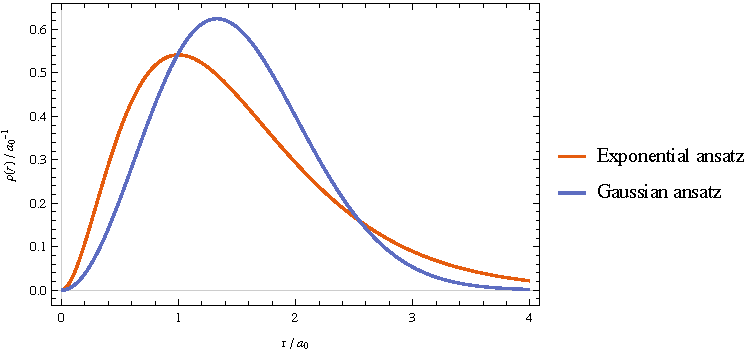
\includegraphics{vary-plt.pdf}
\end{figure}


\paragraph{Appendix: calculating 50th percentile}

\begin{gather}
	4 \pi \int_0^x
	r^2 |\psi_e|^2
	\,\mathrm{d}r
	=
	4 \pi A^2
	\int_0^x r^2 e^{-2(r/a^\star_e)}
	\,\mathrm{d}r
	=
	1
	-
	e^{-2x/a_e^\star}
	\left(
		1
		+
		\frac{2x}{a_e^\star}
		+
		\frac{2x^2}{{a_e^\star}^2}
	\right)
	% =
	% 1-e^{-2\xi}
	% \left(1+2 \xi + 2\xi^2\right)
	=
	\frac{1}{2}
	\implies
	x_\text{50}
	=
	1.337 a_e^\star.
	% \frac{\partial}{\partial r} r^2 e^{-2(r/a)} 
	% = -2 e^{-2(r/a)} r (r-a)/a
	% =
	% 0
	% \implies
	% r = a
	% \\
	% a^2 e^{-2 (a/a)}
	% =
	% \frac{1}{2} \times r_\text{FWHM}^2 e^{-2(r_\text{FWHM}/a)}
	% \implies
\end{gather}
\begin{gather}
	4 \pi \int_0^x r^2 |\psi_g|^2 \,\mathrm{d}r
	=
	4\pi B^2 
	\int_0^x r^2 e^{-2(r/a_g^\star)^2}
	\,\mathrm{d}r
	=
	\mathrm{erf}\left(
		\frac{\sqrt{2}x}{a_g^\star}
	\right)
	-
	\frac{2x}{a_g^\star}\sqrt{\frac{2}{\pi}}
	e^{-2(x/a_g^\star)^2}
	\implies x_{50} = 0.7691 a_g^\star
\end{gather}
The relations between $x_{50}$ and $a^\star$ are found by converting to dimensionless units $x_{50}/a^\star$ and solving numerically.





\end{document}






